\documentclass[a4paper,12pt]{article}

% Packages
\usepackage{graphicx}
\usepackage{amsmath}
\usepackage{amsfonts}
\usepackage{geometry}
\usepackage{fancyhdr}
\usepackage{setspace}
\usepackage{titlesec}  % For title formatting
\usepackage{hyperref}
\usepackage{xcolor}
\usepackage{minted}
\usepackage{dirtytalk}
\usepackage{enumitem}

\setminted[cmake]{
    linenos=false,
    breaklines=true,
    encoding=utf8,
    fontsize=\footnotesize,
    frame=lines
}
\hypersetup{
    colorlinks=true,
    linkcolor=darkgray,
    % filecolor=magenta,      
    % urlcolor=cyan,
    % pdftitle={Overleaf Example},
    % pdfpagemode=FullScreen,
    }
\usepackage{etoolbox}

\AtBeginEnvironment{minted}{\dontdofcolorbox}
\def\dontdofcolorbox{\renewcommand\fcolorbox[4][]{##4}}

% text
\geometry{margin=1in}
\setstretch{1.1}
\setlength{\parskip}{0.8em} 
\setlength{\parindent}{1em} 
\setlist[itemize]{topsep=-6pt, partopsep=0pt, parsep=0pt, itemsep=0pt}

% Header and Footer
\setlength{\headheight}{14.5pt} % Fix for fancyhdr warning
\addtolength{\topmargin}{-2.5pt} % Compensate for increased headheight
\pagestyle{fancy}
\fancyhf{}
\fancyhead[L]{Jocs per Computador}
\fancyhead[R]{\thepage}

% Images settings
\graphicspath{{figs/}}

% Title Formatting
\titleformat{\section}{\normalfont\Large\bfseries}{\thesection}{1em}{}

% Cover Page
\title{
    \vspace{2cm} % Adjust vertical space
    
\includegraphics[width=0.75\textwidth]{fib.png} \\ % Add your logo here (change "logo.png" to the actual filename)
    \vspace{1cm} % Adjust vertical space after the logo
    \textbf{\Huge Jocs per Computador} \\
    \vspace{1cm} % Adjust vertical space
    \large JC-MEI \\
    \vspace{0.5cm} % Adjust vertical space
    \large \today
}
\author{
Carles Matoses Gimenez
    \thanks{
    Email: carles.matoses@estudiantat@upc.edu}\\
Carles Matoses Gimenez
    \thanks{
    Email: carles.matoses@estudiantat@upc.edu}\\
}
\date{
    % \vspace{0.5cm}
    % \textbf{Additional Info:} some info
}

\begin{document}

% Title Page
\maketitle
\thispagestyle{empty}
\newpage

% Table of Contents
% Start page numbering from the Table of Contents
\setcounter{page}{1}  % Start counting from 1
\tableofcontents
\newpage

\section{Introducció}

\section{Objectius}
\subsection{Mapa}
% mostrar imatge del mapa amb el recorregut
\begin{figure}[ht!]
    \centering
    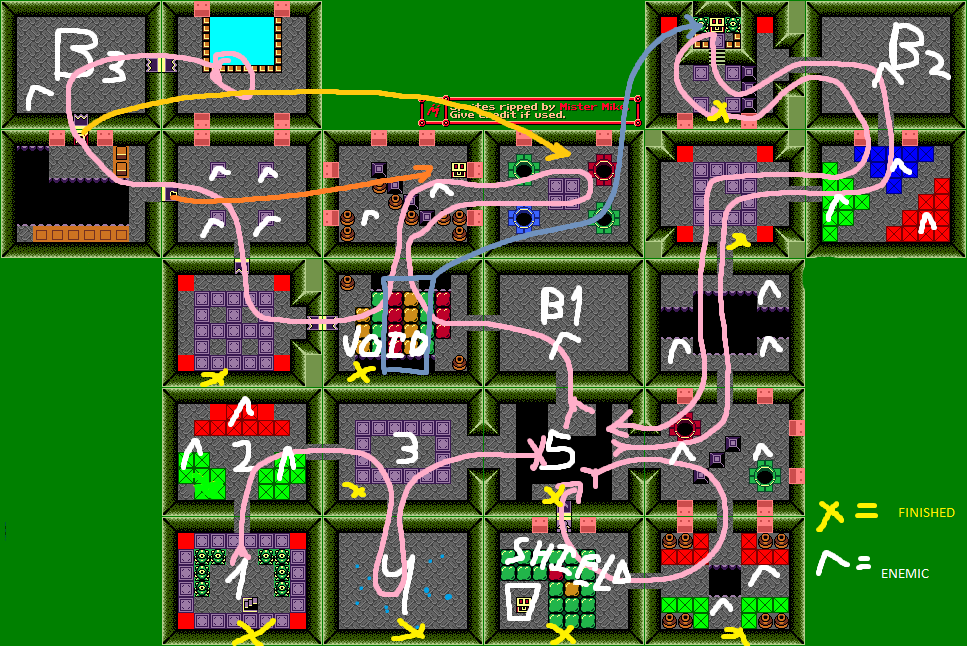
\includegraphics[width=0.8\textwidth]{../imgs/recorregut.png} % Example of adding a figure
    \caption{Mapa del joc amb el recorregut i els requerriments per a  cada nivell.}
    \label{fig:mapa}
\end{figure}

\section{Disseny}
Per al disseny del joc no hem seguit un patró de disseny concret. El ``loop'' del joc incorpora una clase auxiliar que anomenada gamestatemanager. Aquesta conté una llista amb els estats necessaris. L'objectiu de gastar aquesta classe és poder anyadir i eliminar estats dinamicament. Per exemple, qual el jugador apreta ``escape'' i s'obre el menú, el que realment s'està fent és concatenar dos estats i sols permitir que el més alt en la jerarquia puga llegir els inputs i actualitzar-se en funció del temps. 

\subsection{Nivells, elements i entitats}
La classe \texttt{World} guarda un diccionari amb els mapes. La classe \texttt{Mapa} conté una llista amb els nivells. La classe \texttt{Level} contente una llista amb els elements i entitats que s'han de carregar. Per al projecte s'ha creat un World que conte dos mapes, ``dungeon1'' i ``overworld''. El mapa ``dungeon1'' conté 29 nivells. Cada nivell es responsable de contindre els estats per defecte de les entitats i també de customitzar events com "entrar" i "sortir" de les entitats. 


\begin{figure}[ht!]
    \centering
    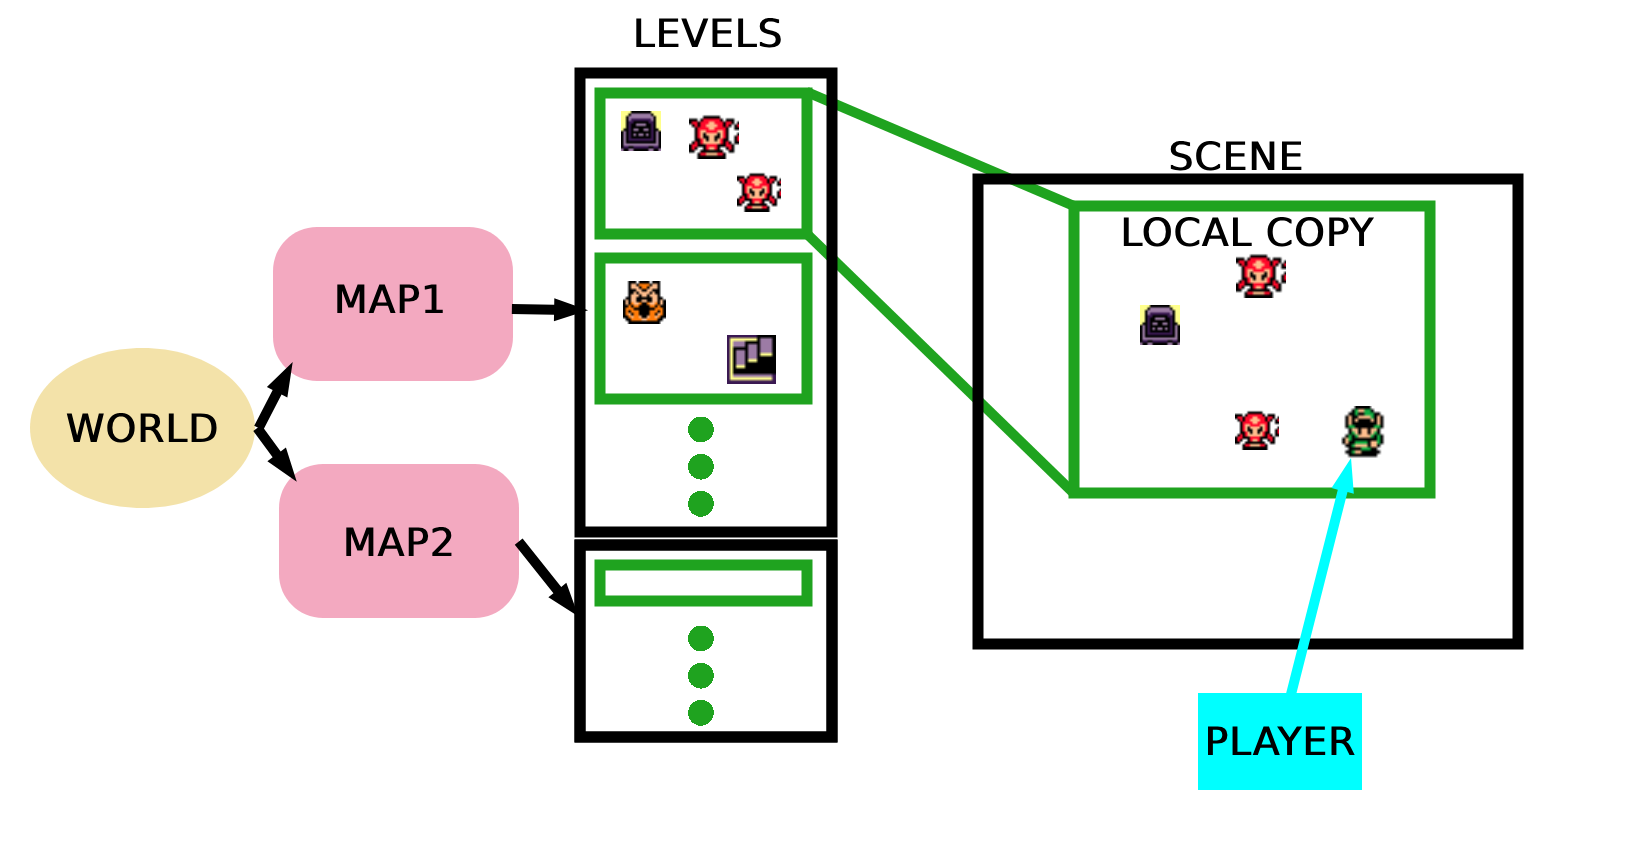
\includegraphics[width=0.8\textwidth]{../imgs/global_to_local.png} % Example of adding a figure
    \caption{Jerarquia dels elements durant l'execució del joc.}
    \label{fig:global_to_local}
\end{figure}

\subsection{Mecàniques}
\subsection{Triggers}
% onEnter
% onExit
% onAllEnemyesDead

\section{Trenca closques}

\section{Enemics}



\section{Examples}
Code examples:
\subsection{Text}
 Lorem ipsum dolor sit amet, consectetur adipiscing elit. Donec sit amet arcu aliquam, mattis sapien quis, faucibus ligula. Praesent facilisis felis libero, nec scelerisque est vestibulum a. Proin gravida tempor neque eget maximus. Aliquam vel ex arcu. Maecenas porta blandit leo, eget dapibus libero faucibus quis. Curabitur vel sapien pharetra, ultricies nulla sed, ullamcorper metus. Sed mauris sapien, dapibus et elit in, bibendum pellentesque dui. Donec consequat quam ut pulvinar sodales. Duis commodo ex pharetra mauris dictum, in ultricies purus facilisis. Donec id ornare sem. Nam diam erat, imperdiet et orci id, lacinia condimentum justo. Integer laoreet pulvinar nibh. Vivamus vel tellus lacus.

\begin{itemize}
    \item one
    \item one
    \item one
    \item one
    \item one
    
\end{itemize}

Phasellus congue, massa in aliquet elementum, ipsum felis dictum enim, id maximus ante orci sit amet dui. Suspendisse blandit iaculis feugiat. Curabitur ante elit, tristique luctus hendrerit sed, posuere quis massa. Vivamus eu nunc vel neque egestas porttitor ac at nibh. Morbi odio justo, maximus sit amet elementum nec, finibus sed purus. Mauris eu posuere neque, at consequat elit. Praesent eu venenatis mauris, vel lobortis eros. Donec suscipit congue augue, ut aliquet metus volutpat ac. Vivamus mattis, nisl vel placerat euismod, tellus velit sollicitudin massa, nec sagittis nunc elit vel mauris. In id justo non nunc condimentum bibendum. Mauris scelerisque urna nisi, et lacinia justo posuere eget. 
\begin{figure}[ht!]
    \centering
    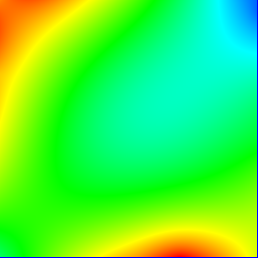
\includegraphics[width=0.8\textwidth]{img/eg.png} % Example of adding a figure
    \caption{Test results for circuit 1}
    \label{fig:circuit1}
\end{figure}

\begin{figure}[ht!]
    \centering
    \begin{minipage}{0.30\linewidth}
        \centering
        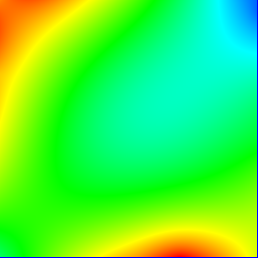
\includegraphics[width=\linewidth]{img/eg.png}
        \caption{subimage1}
        \label{fig:subimage1}
    \end{minipage}
    % \hfill
    \begin{minipage}{0.30\linewidth}
        \centering
        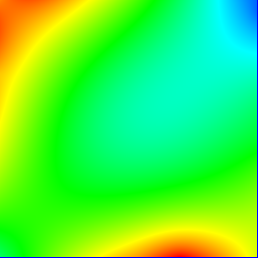
\includegraphics[width=\linewidth]{img/eg.png}
        \caption{subimage2}
        \label{fig:subimage2}
    \end{minipage}
\end{figure}


\subsection{Code}
\begin{minted}{c}
#define NB 2 // selected based on the number of threads
...
double relax_jacobi (double *u, double *utmp, unsigned sizex, unsigned sizey)
{
...
    #pragma omp parallel for reduction(+:sum) private(diff)
    for (int ii=0; ii<nbx; ii++) {
        ...
    }
    return sum;
}
\end{minted}

\newpage
% Bibliography (if required)
% Example citation to avoid warning
\nocite{*}
\bibliographystyle{plain}
\bibliography{references}  % Add a .bib file if you have references

\end{document}

\end{document}
